\chapter{Hardware}\label{ch:hardware}

\paragraph{Hardware in the device} 



In the following chapter we will see what hardware we have used to produce this device.
First we decided on what platform we will be working on.

\section{Single board computer} 

Since we were allready familiar with the Raspberry Pi singleboard computer we decided that it is best to continue with the system we are allready know how to operate.
At first we used the Raspberry Pi 2 model B but in concideration of the power supply and performance we swapped it out with a Raspberry Zero.


\begin{figure}[h]
\centering
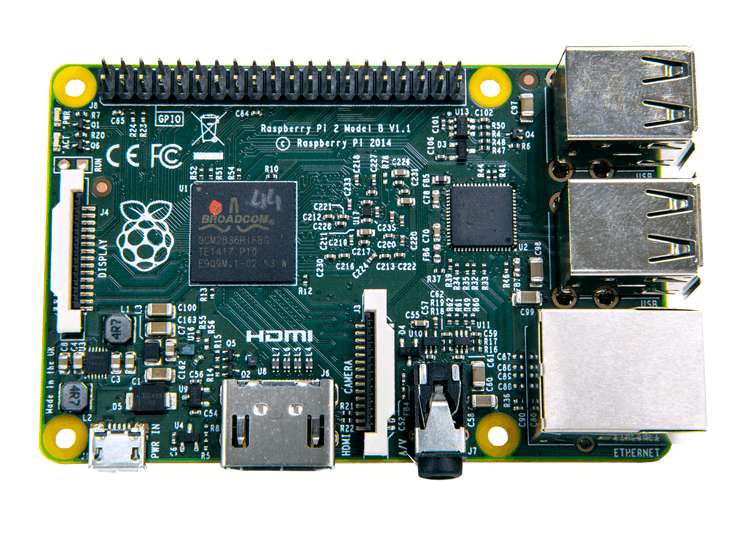
\includegraphics[width = 0.5\textwidth]{Raspberry-Pi-2}
\caption{Raspberry Pi 2B}
\label{fig::rasppi2b}
\end{figure}

\begin{figure}[h]
\centering
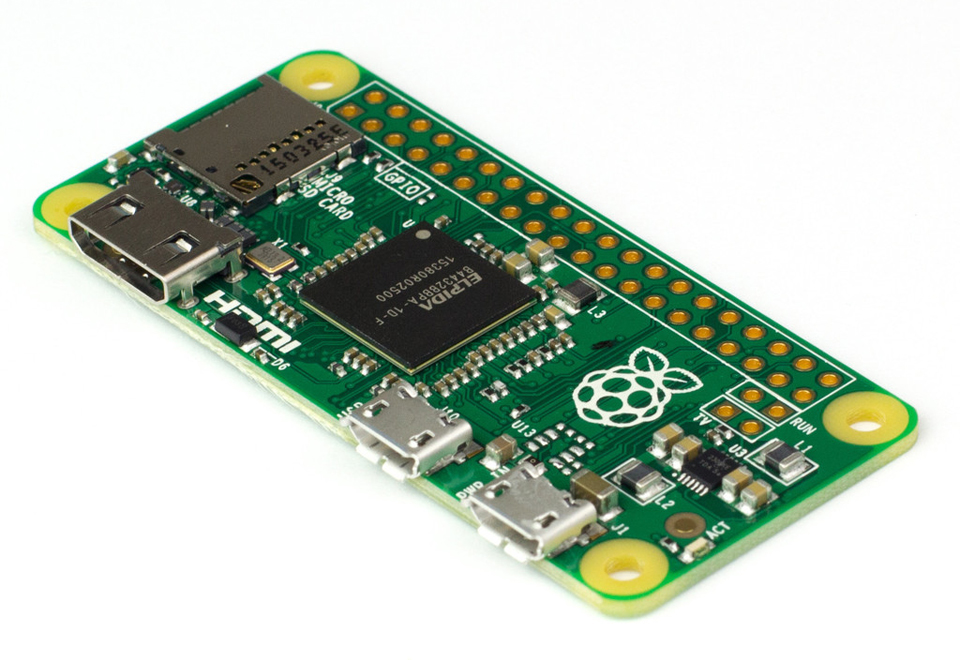
\includegraphics[width = 0.5\textwidth]{raspberry_pi_zero_1}
\caption{Raspberry Pi Zero}
\label{fig::raspizero}
\end{figure}


We chose the Rasperry Pi Zero over the Raspberry Pi 2B because of the lesser power consumption and the size.
Performance of the two computers are similar. 
Zero has less RAM but in our project it does not have a significant impact.

Specs of the Raspberry Pi Zero:
1Ghz, Single-core CPU
512MB RAM
Mini HDMI and USB On-The-Go ports
Micro USB power
HAT-compatible 40-pin header
Composite video and reset headers



\section{Distance measuring} 

Since our device would be avoiding obstacles on the way it is fitted with distance measuring sensors.
We have decided to use ultra sonic sensors.
Concidering the cost and the performance we are looking for we eventually settled on the HC-SR04 ultra sonic sensor.
In our device we have used three of those sensors in orded to cover the front side of the veichle.

\begin{figure}[h]
\centering
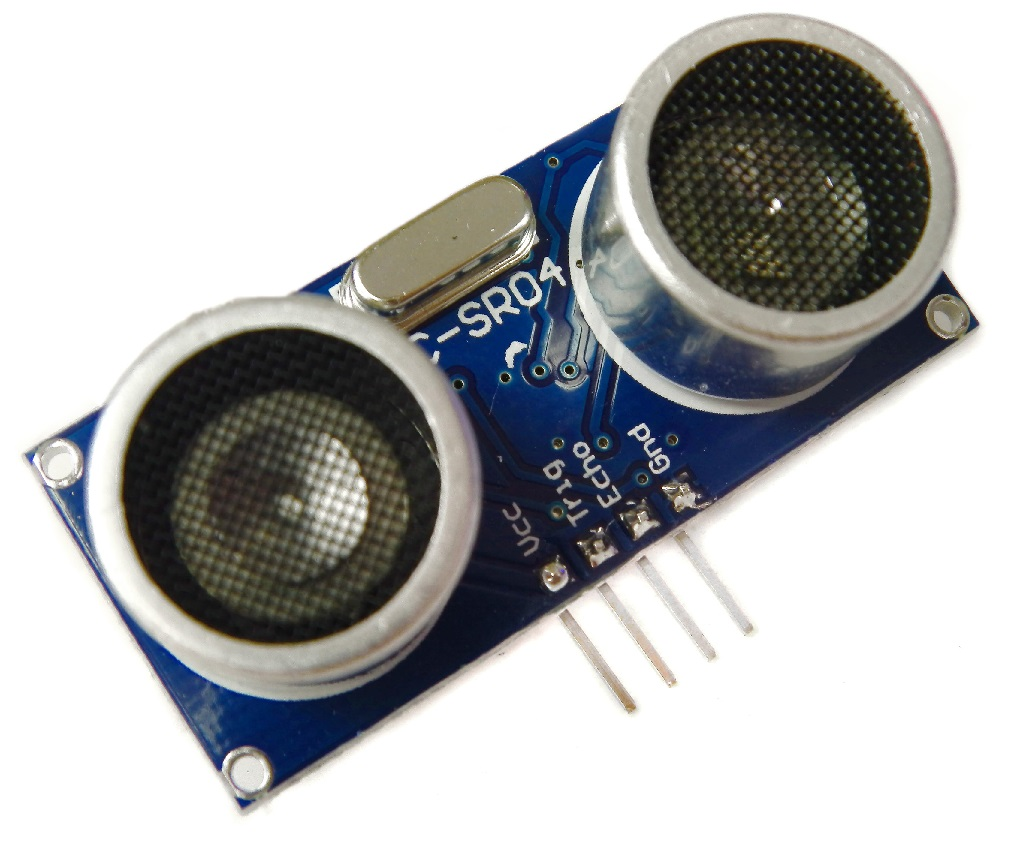
\includegraphics[width = 0.5\textwidth]{hc-sr04}
\caption{Ultra sonic sensor HC-SR04}
\label{fig::hcsr04}
\end{figure}

\section{DC motors and the chassie} 

We are using a premade complect of two DC motors and the chassie with the wheels.
Each of the motors are connected to the wheels directly.

\begin{figure}[h]
\centering
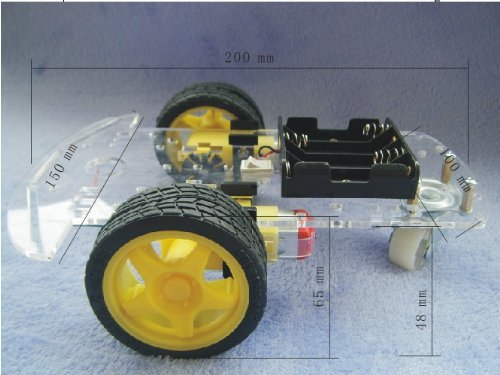
\includegraphics[width = 0.5\textwidth]{chassie}
\caption{Chassie and the two DC motors with a power supply}
\label{fig::chassie}
\end{figure}

Motor specs:

 Voltage:
DC 3V
DC 5V
DC 6V
Current:
100 MA
100MA
120MA
Reduction rate:48:1
RPM (With tire):100,190,240
Tire Diameter:66mm
Car Speed(M/minute):20,39,48

Motor Weight (g):50

Motor Size:70mm*22mm*18mm

Noise:<65dB 

(CITE: https://elektronik-lavpris.dk/p129700/robo0002-smart-robot-car-chassis-kit-with-speed-encoder-and-battery-box/)
The two motors are identical and are used to move the device and to steer aswell

\section{Motor driver} 

At the beginning of the project we used a L9110S DC Stepper Motor Driver H-Bridge for controlling the movement of the wheels, but as we soon dicovered the suggested driver was not capable of regulating the motor speeds.
To controll the speed of the veichle we then swapped it to the L298N driver.
The second driver was capable of using the PWM to regulate the speed of the motors.

\begin{figure}[h]
\centering
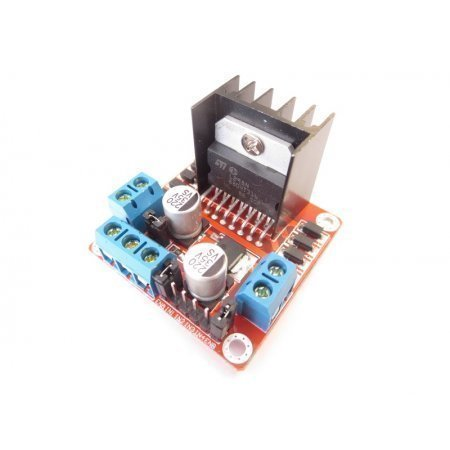
\includegraphics[width = 0.5\textwidth]{driver2}
\caption{The L298N driver}
\label{fig::driver2}
\end{figure}

Driver specs:
Working mode:	H bridge (double lines)
Control chip:	L298N (ST)
Logical voltage:	5V
Driving voltage:	5V-35V
Logical current:	max 36mA
Driving current:	2A (max single bridge)
Maximum power:	25W
Storage temperature:	-20 °C +135 °C
Periphery dimension:	43 x 43 x 27mm(L x W x H)

\section{Speed sensor}

The speed of the wheels is measured by the LM393 IR speed sensors.

\begin{figure}[h]
\centering
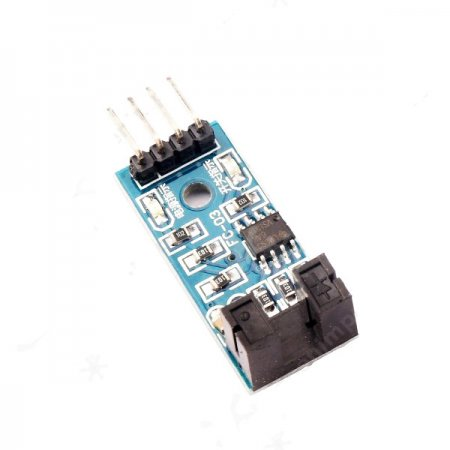
\includegraphics[width = 0.5\textwidth]{irspeed}
\caption{The LM393 IR speed sensor}
\label{fig::driver2}
\end{figure}

The speed sensor is used to estimate the error of the wheel speed.
Features:

Working voltage: 3.3V~5V
Weight: 8g
Dimensions: Approx.3.2 x 1.4 x 0.7cm
5mm Groove width
Using wide voltage LM393 comparator
Application: Widely used in dynamo speed detecting, pulse counting, etc
Output form: Digital switch output (0 and 1) and Analog for Sensitivity.
(CITE:http://www.banggood.com/LM393-Speed-Sensor-Detection-Speed-Module-For-Arduino-p-970033.html?currency=AUD&utm_source=myshopping&utm_medium=cpc&utm_content=saul&utm_campaign=xie-AU)

\section{Wi-Fi dongle}

For the monitoring of the device and connectivity we have used a Edimax EW-7811Un Wi-Fi adapter.

\begin{figure}[h]
\centering
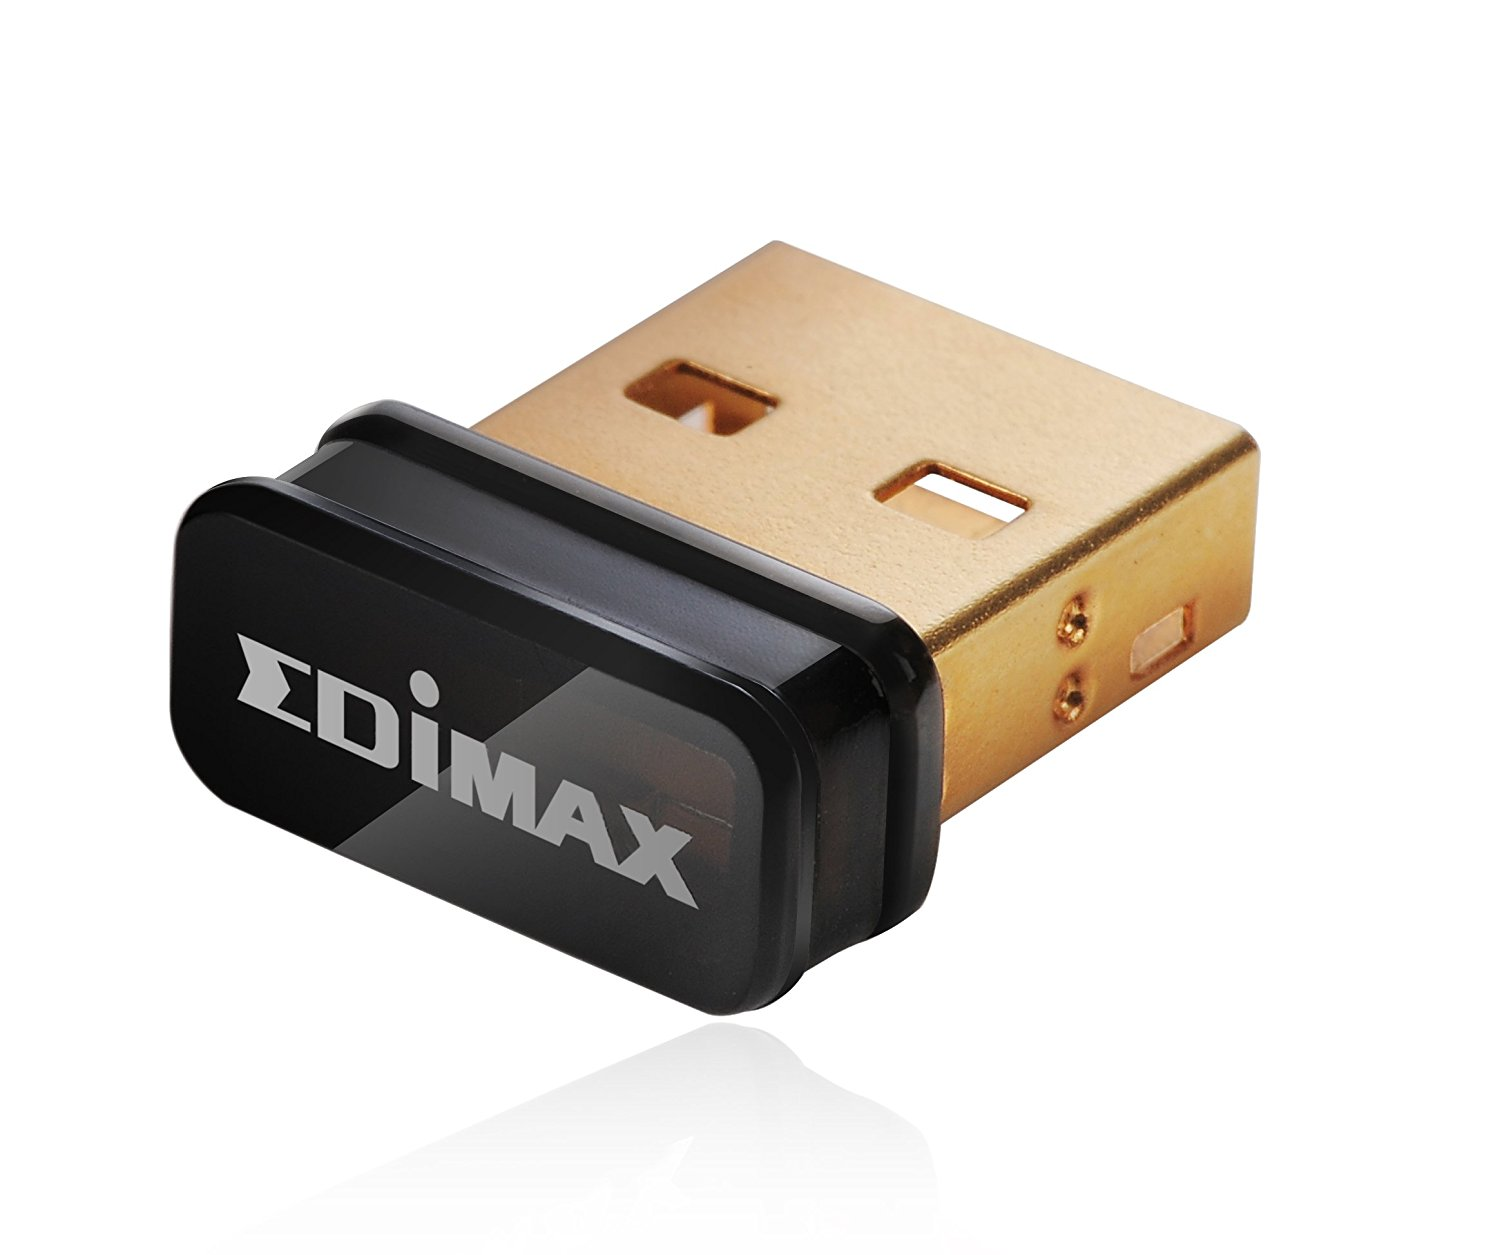
\includegraphics[width = 0.5\textwidth]{edimax}
\caption{Edimax EW-7811Un Wi-Fi adapter}
\label{fig::edimax}
\end{figure}

\section{Assambly}

In this section we will be looking more closely what has been connected to what and how.
From the figure below we can see the layout of the whole system.

\begin{figure}[h]
\centering
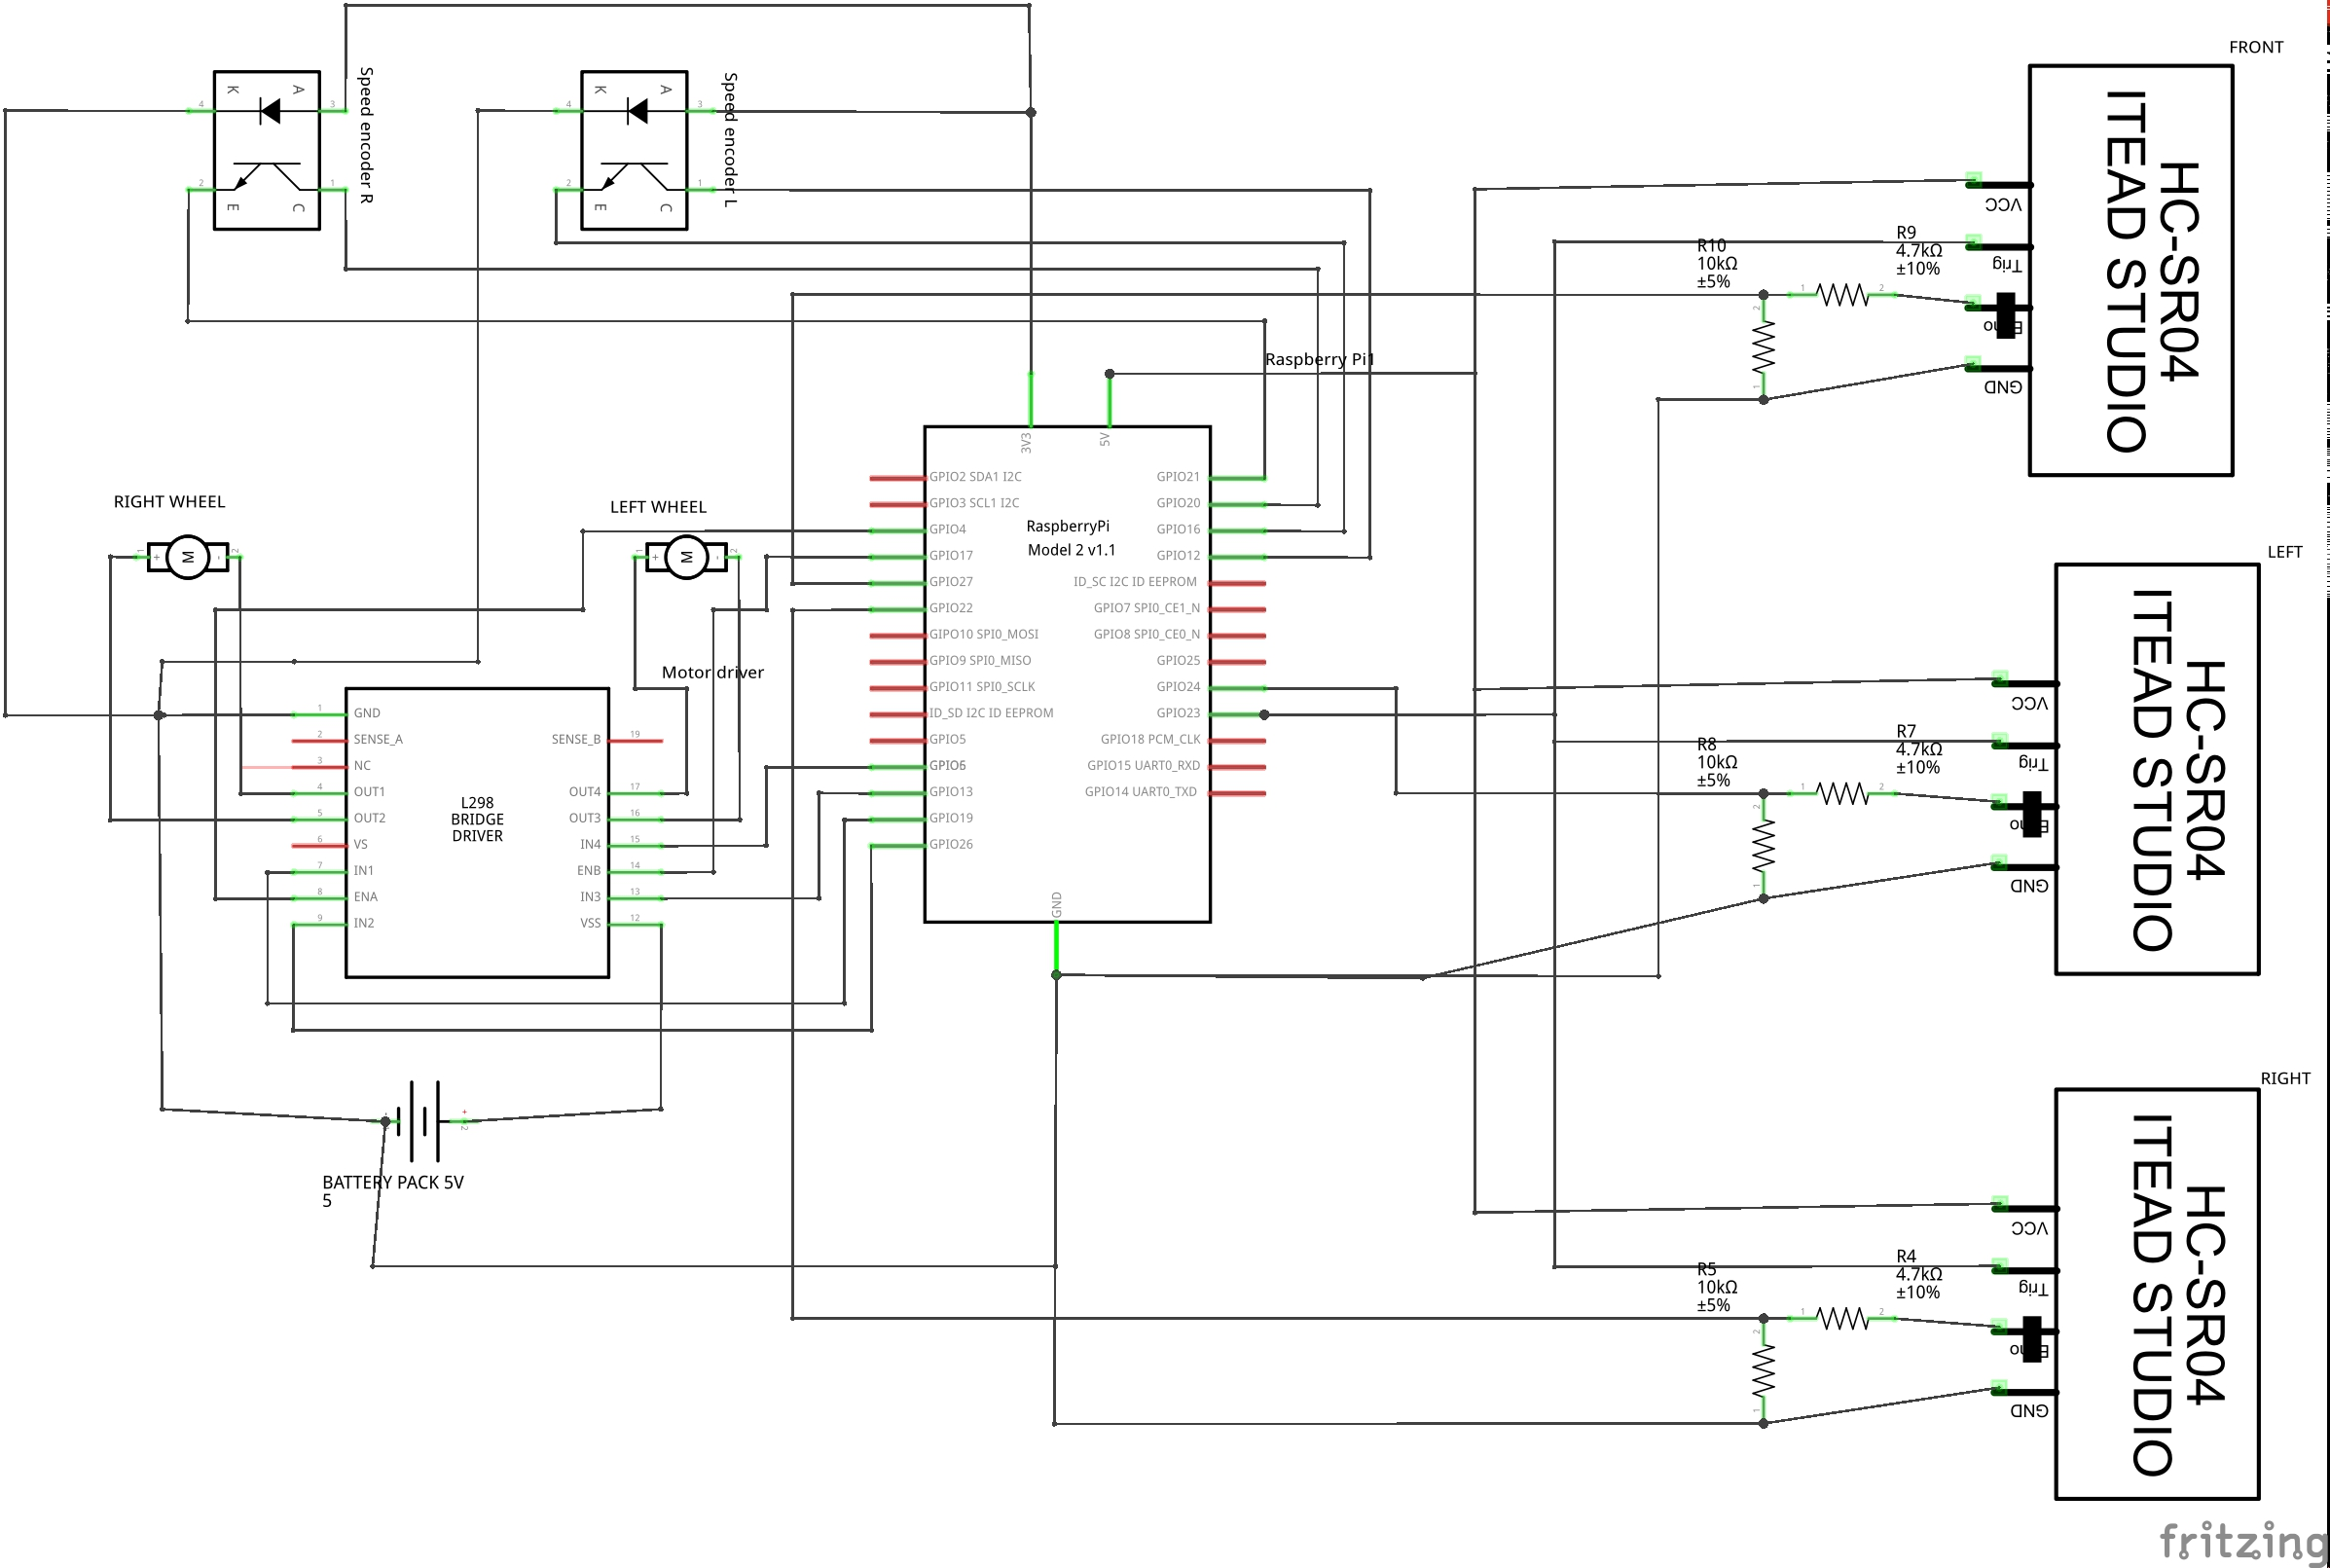
\includegraphics[width = 0.5\textwidth]{P51_schem}
\caption{Schematics of the device}
\label{fig::schematics}
\end{figure}

In the middele you can see the Raspberry Pi.
Since the software used to make this schematic did not have the Raspberry Pi Zero layout we used model 2 instead.
Regarding our project id does not make a difference, since the pins are the same as Zero.

On the right side of the system you can see three ultrasonic sensors.
The ultrasonic sensors are connected to the RP Pi.
The Vcc and GND pins all go to the Raspberry so that the power for the sensors is taken from the Raspberry itself.
The triger pins all go to the same Raspberry pin.
That means that when you trigger one of the sensors all of them will emit sonic impulse.
The trigers are all on the same pin to preserv more pins on the Raspberry, it does not matter if they are on one or seperate pins.
The echo pins of each of the sensors go into seperate ports on the Raspberry, each of them has a voltage divider connected to the GND as well.

In the left bottom you can see the driver with the motors and a seperate battery pack.
The battery pack is connected to the driver to give power to the motors and the driver itself aswell.
Driver is connected to the Raspberry by 6 pins.
Four of the pins are for the directions of the both motors.
Two of the pins what are the enable pins are used for controlling the speed of the motors by PWM.
The motors are connecter directly to the driver by two wires.
In the top left you can see the two encoders what are used for monitoring the speed of the wheels.

For the Raspberry we have a external power source what is not pictured on the figure.

